\mkexercise{El circuito de la figura muestra el esquema de
construcción de dos señales suma $V_{suma}(t) = V_{Der}(t) + V_{Izq}$
y resta $V_{resta}(t) = V_{Der}(t) - V_{Izq}$ correspondientes a los
canales derecho $V_{Der}(t)$ e izquierdo $V_{Izq}(t)$ de una señal FM
estéreo compatible. Esta operación es un estándar que permite
reproducir señales estéreo en receptores de radio estéreos con dos
altavoces, y señales monoaurales en receptores de radio con un solo
altavoz. El circuito se ha construido en el simulador con la librería
matemática ABM.OLB usando los operadores Suma (SUM) y diferencia
(DIFF).

    \begin{figure}[H]
    \centering  
    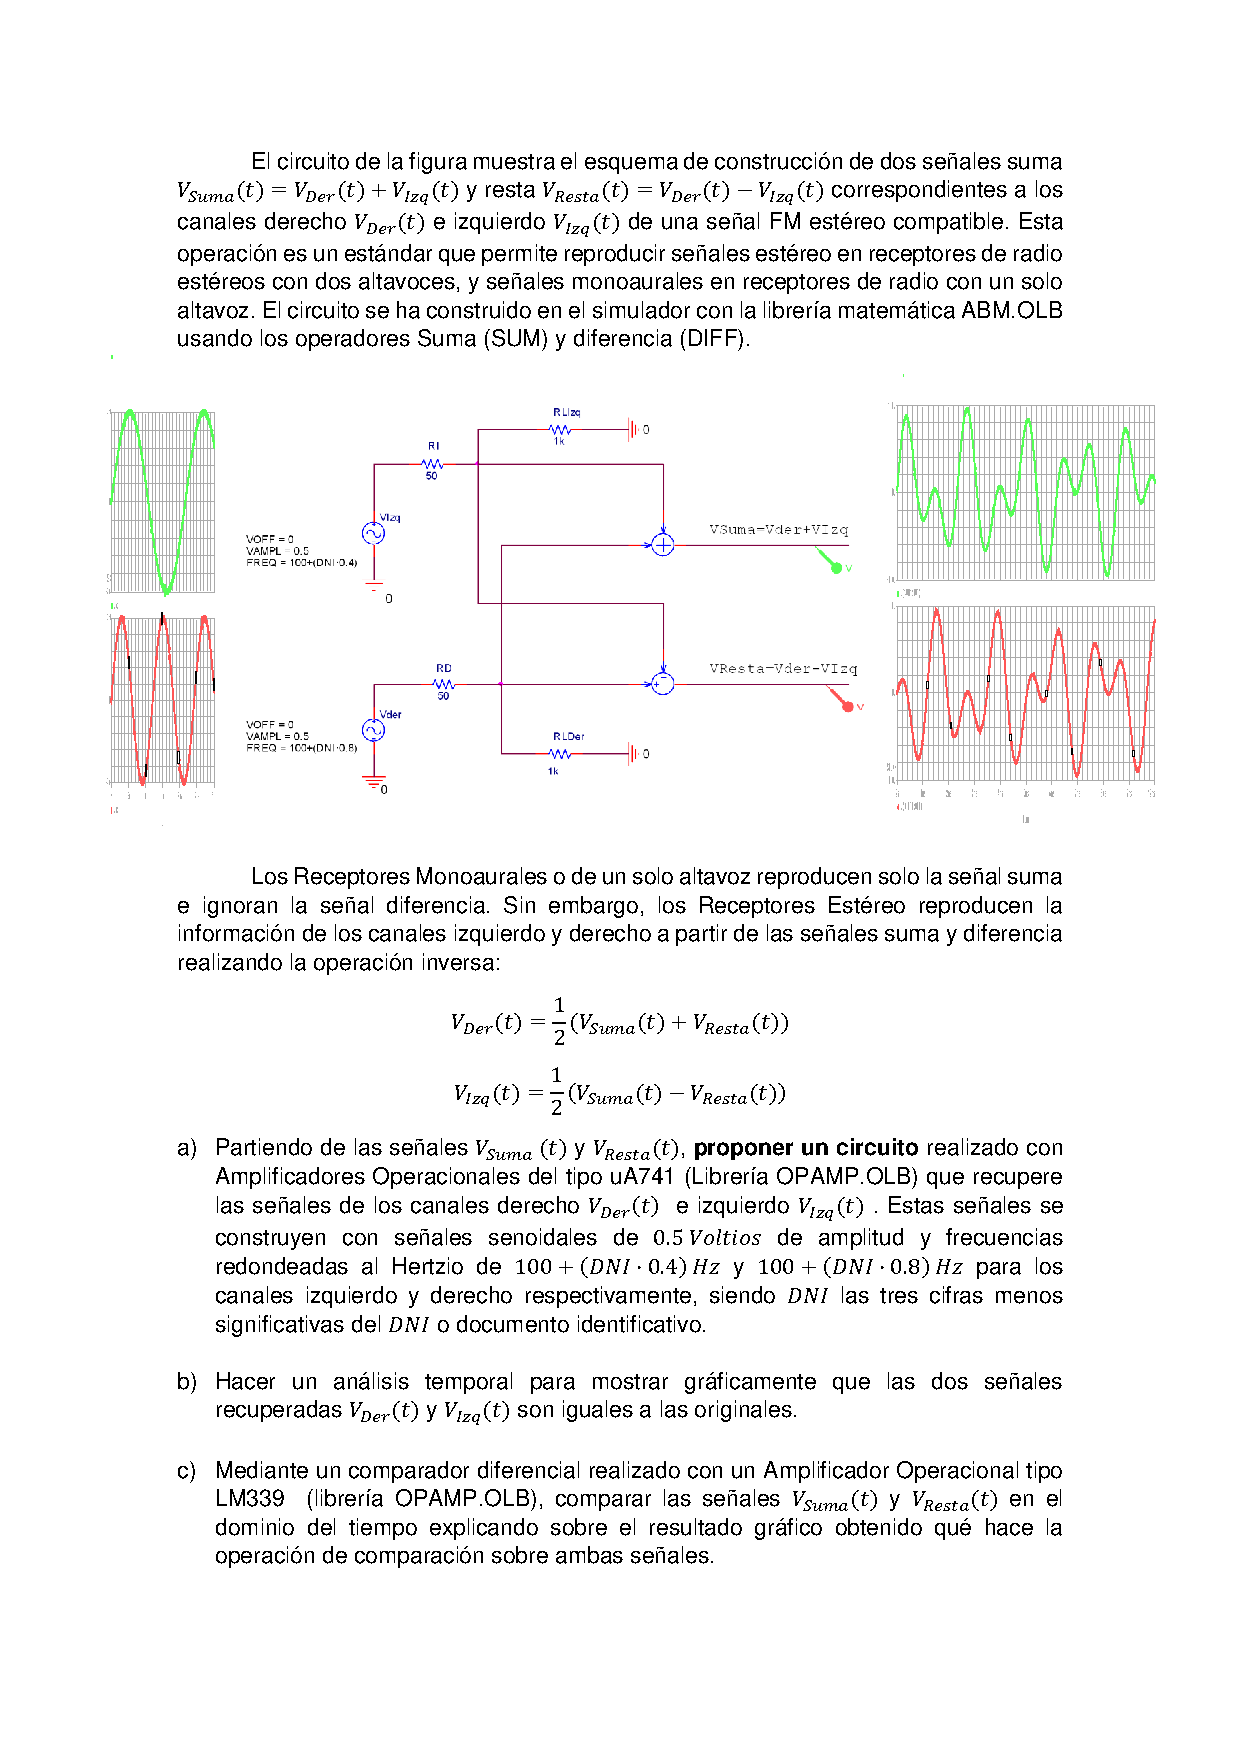
\includegraphics[scale=0.5,page=1,clip, trim=0cm 16cm 0cm 6cm]{images/problema_puntuable_6.pdf}
    % izquierda,abajo,derecha,arriba
    \caption{Circuito inicial}
  \end{figure}


Los Receptores Monoaurales o de un solo altavoz reproducen solo la
señal suma e ignoran la señal diferencia. Sin embargo, los Receptores
Estéreo reproducen la información de los canales izquierdo y derecho a
partir de las señales suma y diferencia realizando la operación
inversa:
\begin{equation}
    V_{Der}(t) = \dfrac{1}{2}\left(V_{Suma}(t)+V_{Resta}(t)\right)\\
\label{equa1}
  \end{equation}

  \begin{equation}
        V_{Izq}(t) = \dfrac{1}{2}\left(V_{Suma}(t)-V_{Resta}(t)\right)\\
\label{equa2}
      \end{equation}

\begin{itemize}

\item Partiendo de las señales $V_{Suma}(t)$ y $V_{Resta}(t)$,
proponer un circuito realizado con Amplificadores Operacionales del
tipo $\mu A741$ (Librería OPAMP.OLB) que recupere las señales de los
canales derecho $V_{Der}(t)$ e izquierdo $V_{Izq}(t)$ .

Estas señales se construyen con señales senoidales de $0.5 V$ de
amplitud y frecuencias redondeadas al Hertzio de $100 + (DNI \cdot 0.4)
Hz$ y $100 + (DNI \cdot 0.8) Hz$ para los canales izquierdo y derecho
respectivamente, siendo DNI las tres cifras menos significativas del
$DNI$ o documento identificativo.

\item Hacer un análisis temporal para mostrar gráficamente que las dos
  señales recuperadas $V_{Der}(t)$ y $V_{Izq}(t)$ son iguales a las
  originales.

\item Mediante un comparador diferencial realizado con un Amplificador
  Operacional tipo LM339 (librería OPAMP.OLB), comparar las señales
  $V_{Suma}(t)$ y $V_{Resta}(t)$ en el dominio del tiempo explicando sobre el
  resultado gráfico obtenido qué hace la operación de comparación
  sobre ambas señales. 
\end{itemize}
}
\newpage
\mksolution{
  Las dos señales con las que tengo que trabajar dado el $DNI = 948$ son:
  \begin{itemize}
  \item $100+(948 \cdot 0.4) = 479.2 Hz$
  \item $100+(948 \cdot 0.8) = 858.4 Hz$
  \end{itemize}

  Para resolver el problema de diseño usaremos las ecuaciones que nos
  da el ejercicio.

  $V_{Izq}$ precisa de una configuración diferencial con ganacia
  $0.5$, en el A.O. introduciremos la suma y la resta como indica la
  ecuación \ref{equa2} y haremos una diferencia, para evitar el uso de
  otro A.O. haremos la operación inversa $V_{Resta}-V_{Suma}$ así la
  señal salida estará en fase con la señal $V_{Izq}$. El uso de
  A.O. no tiene una complejidad excesiva cuando conoces las topologías
  para lograr operaciones matemáticas pero si implica conocer ciertas
  características que ayudan a un mejor funcionamiento de la función
  electrónica, en este caso la ganancia del A.O se puede conseguir con
  cualquier múltiplo de $\dfrac{1}{2}$ esto implica que con
  resistencias de miles de ohmios ya podríamos efectuar las
  operaciones pero el circuito sería mucho más eficiente si usamos
  resistencia más altas para minimizar la caída de tensión en RS, por
  ejemplo podemos usar $8k\Omega$.

  Para obtener $V_{Der}(t)$ podemos hacer uso de varias
  configuraciones pero la más óptima es restar a la suma $V_{Izq}$ ya
  que nos ahorra A.O. y un par de resistencias frente a otras
  configuraciones.

      \begin{figure}[H]
    \centering  
    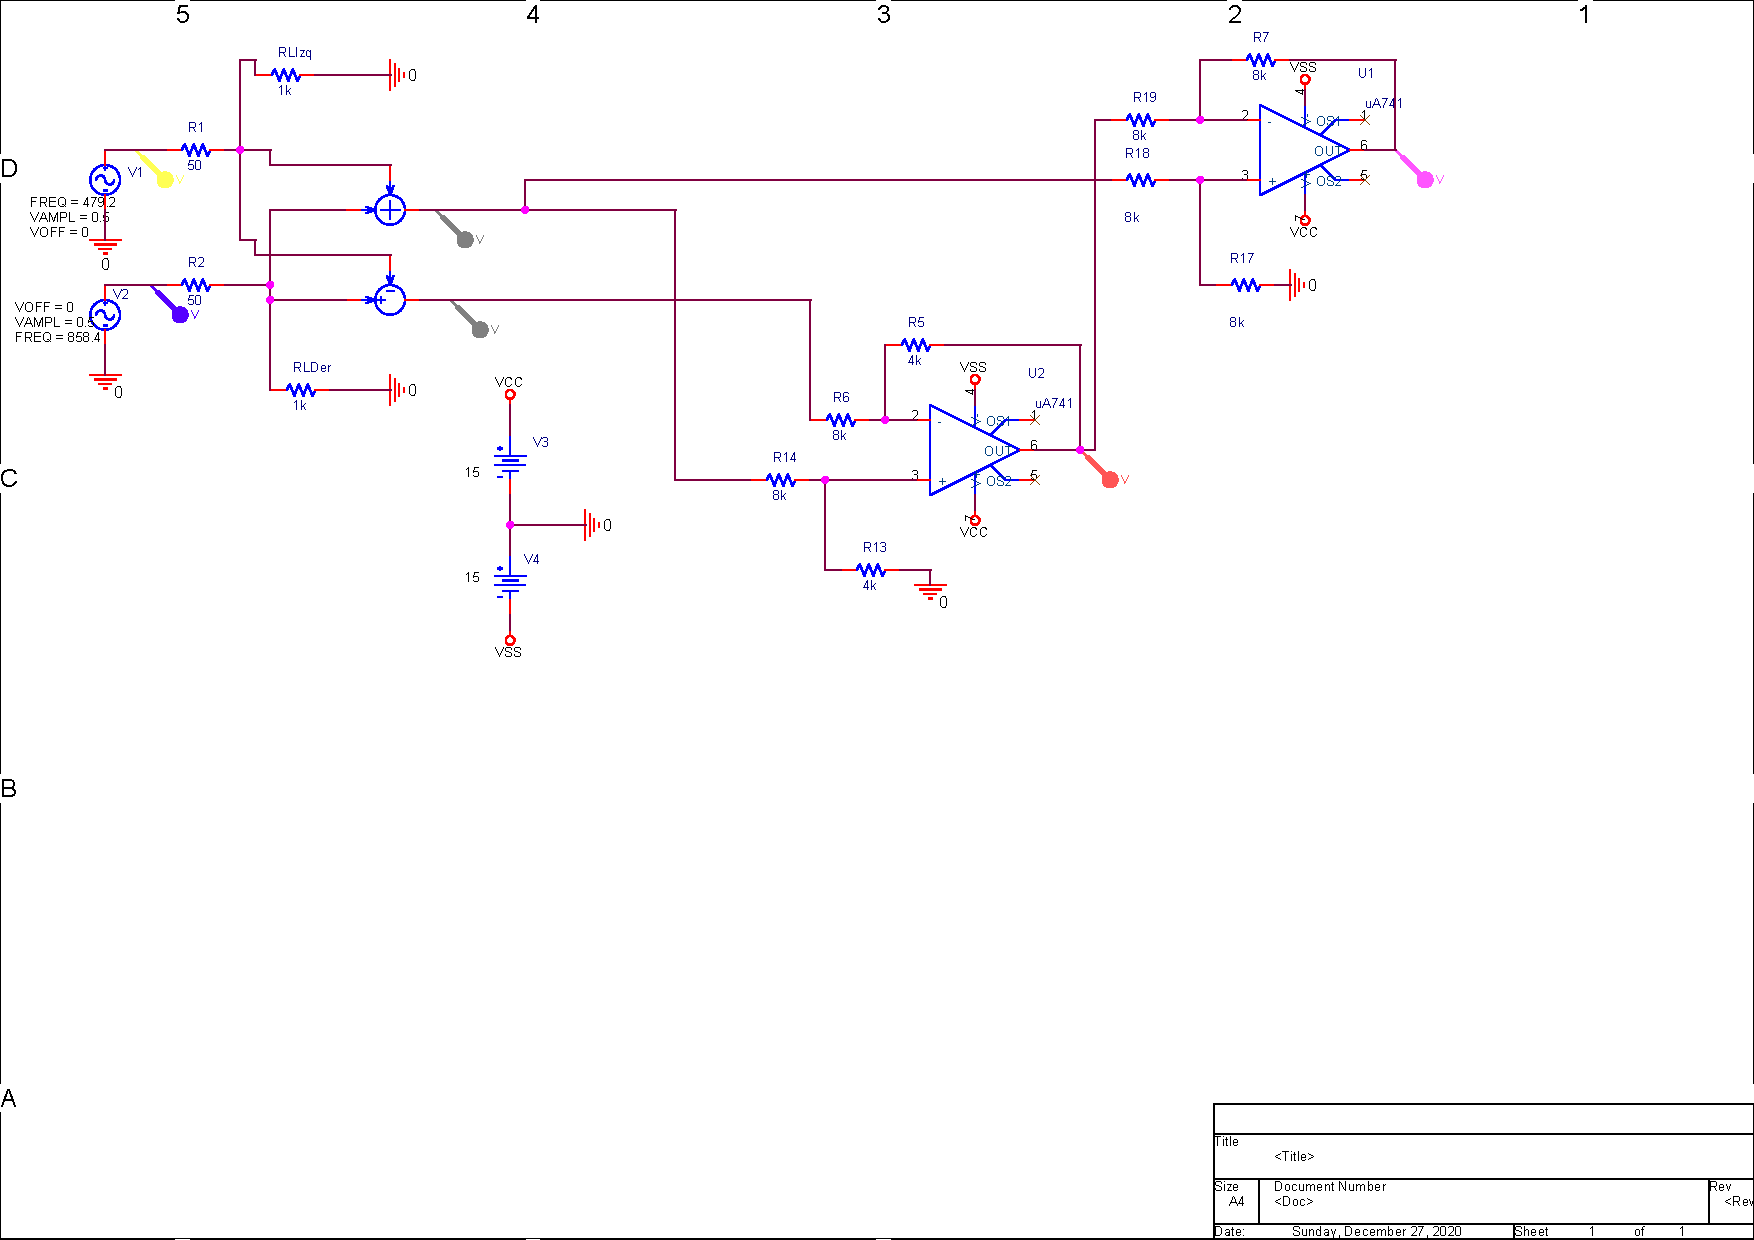
\includegraphics[scale=0.65,page=1,clip, trim=0.4cm 9.5cm 5cm 0.45cm]{images/problema_puntuable_6_sch.pdf}
    % izquierda,abajo,derecha,arriba
    \caption{Solución esquemática del circuito}
  \end{figure}

  En las siguientes imágenes podemos ver algunas respuestas temporales.
    \begin{figure}[H]
    \centering  
    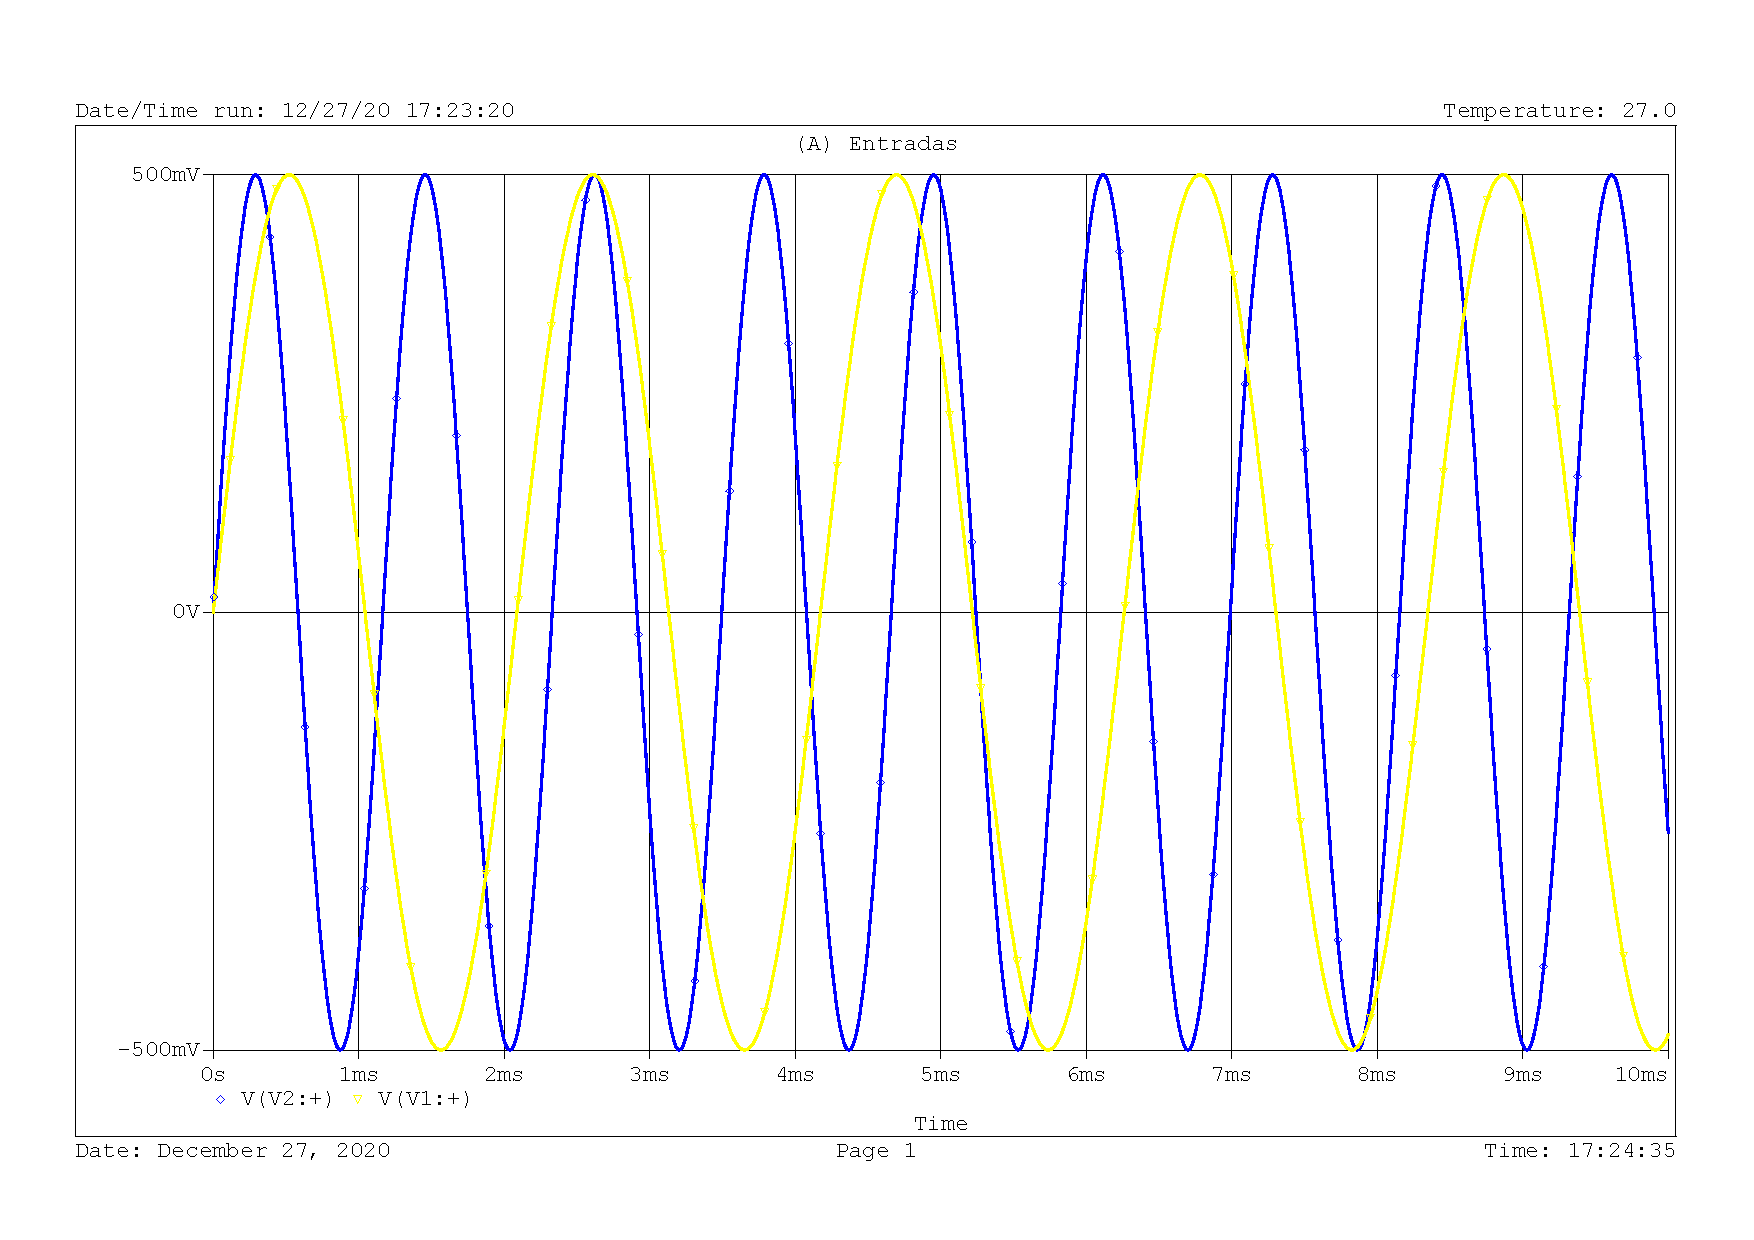
\includegraphics[scale=0.5]{images/problema_puntuable_6_entrada.pdf}
    % izquierda,abajo,derecha,arriba
    \caption{Señales de entrada}
  \end{figure}
  Las entradas que podemos ver en la imagen son las funciones
  senoidales calculadas en las primeras líneas con $DNI$.
  \begin{figure}[H]
    \centering  
    \includegraphics[scale=0.5,page=2]{images/problema_puntuable_6_suma_resta_individual.pdf}
    % izquierda,abajo,derecha,arriba
    \caption{Señal de salida suma}
  \end{figure}

      \begin{figure}[H]
    \centering  
    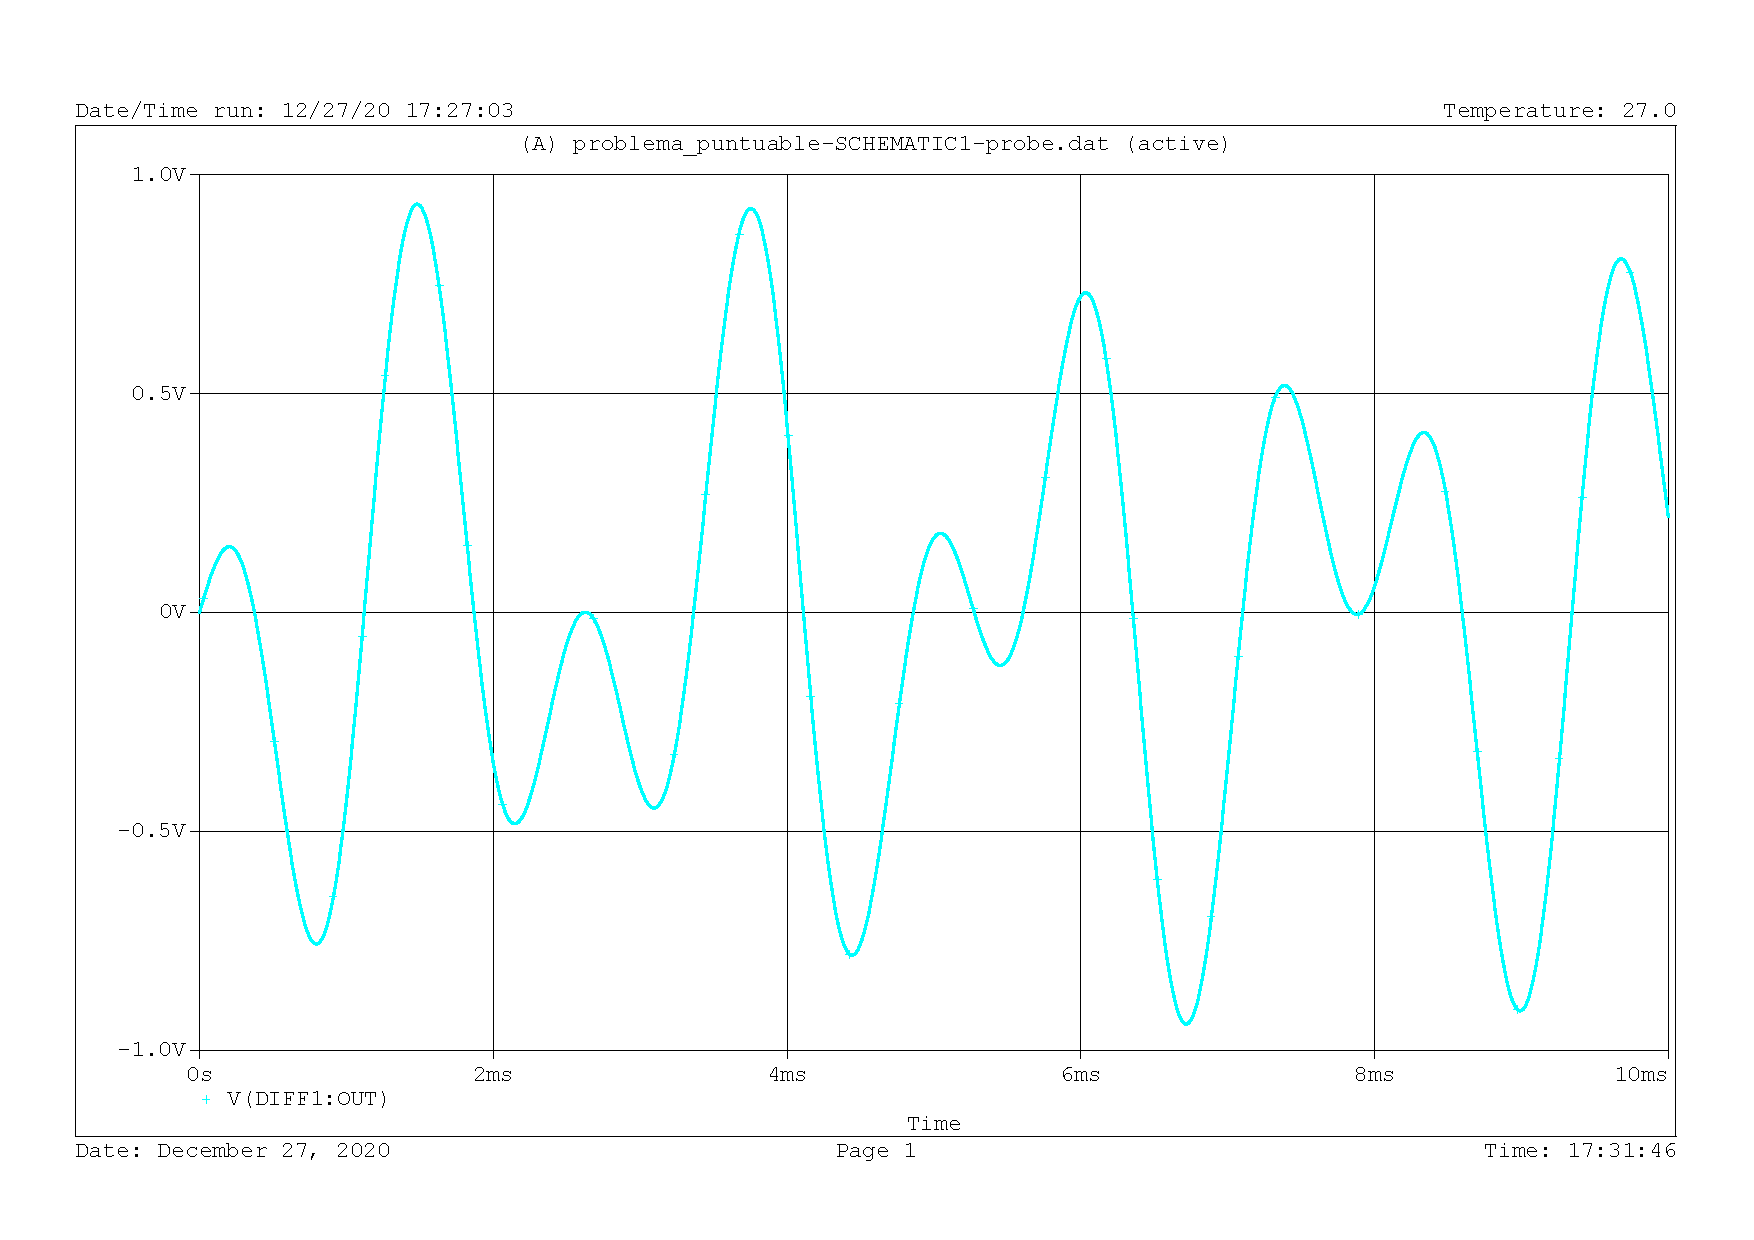
\includegraphics[scale=0.5,page=1]{images/problema_puntuable_6_suma_resta_individual.pdf}
    % izquierda,abajo,derecha,arriba
    \caption{Señal de salida resta}
  \end{figure}

  Obseramos que las señales de salida son idénticas a las que indica
  el enunciado.
  
  \begin{figure}[H]
    \centering  
    \includegraphics[scale=0.5,page=1]{images/problema_puntuable_6_solución_final.pdf}
    % izquierda,abajo,derecha,arriba
    \caption{Entrada - Salida Derecha}
  \end{figure}

      \begin{figure}[H]
    \centering  
    \includegraphics[scale=0.5,page=2]{images/problema_puntuable_6_solución_final.pdf}
    % izquierda,abajo,derecha,arriba
    \caption{Entrada - Salida Izquierda}
  \end{figure}


  Como podemos observar en la imagen las salidas son prácticamente
  iguales, si hay algún retardo es imperceptible, aunque si podemos
  destacar que hay una reducción significativa en la salida, entre los
  30 y 20 $mV$.
}

\mksolution{

Para usar un A.O. como comparador debemos quitar la resistencia $R_1$
y poner un hilo esto nos daría una ganancia infinita lo que se traduce
en que una ligera diferencia en las entradas se multiplicarán por una
gran cantidad lo que da como resultado que el amplificador se sature a
una tensión próxima a la alimentación, esto nos da dos estados de
funcionamiento.

El fabricante (en la página 12) nos da dos configuraciones de uso del
comparador $LM339$, el uso de un dispositivo comparador frente a un
amplificador operaciones con $R_1$ es que la estructura interna del
comparador está diseñada para la comparación a diferencia de un
A.O. con aplicaciones genéricas.

El uso de alguna de las dos configuraciones implica usar una
resistencia conocida como $R_{pullup}$ y un condensador $C_L$ que
condicionan el tiempo de subida y de baja de acuerdo a las siguientes
expresiones:
\begin{equation}
  \begin{split}
    \tau_{subida}& \simeq R_{pullup}\cdot C_L\\
    \tau_{bajada} & \simeq 100 \Omega \cdot c_L\\
    \end{split}
  \end{equation}
  Estos tiempos de subida para generar una señal digital deben ser
  mínimos ya que nuestro interés radica en una rápida conmutación.

  Tenemos unos parámetros de diseño dados por el fabricante que
  debemos cumplir, por lo tanto las especificaciones que usaremos para
  nuestro comparador son:   $R=1k\Omega$ y un $C = 1nF$, 5V en configuración no
  simétrica.

  \begin{figure}[H]
    \centering  
    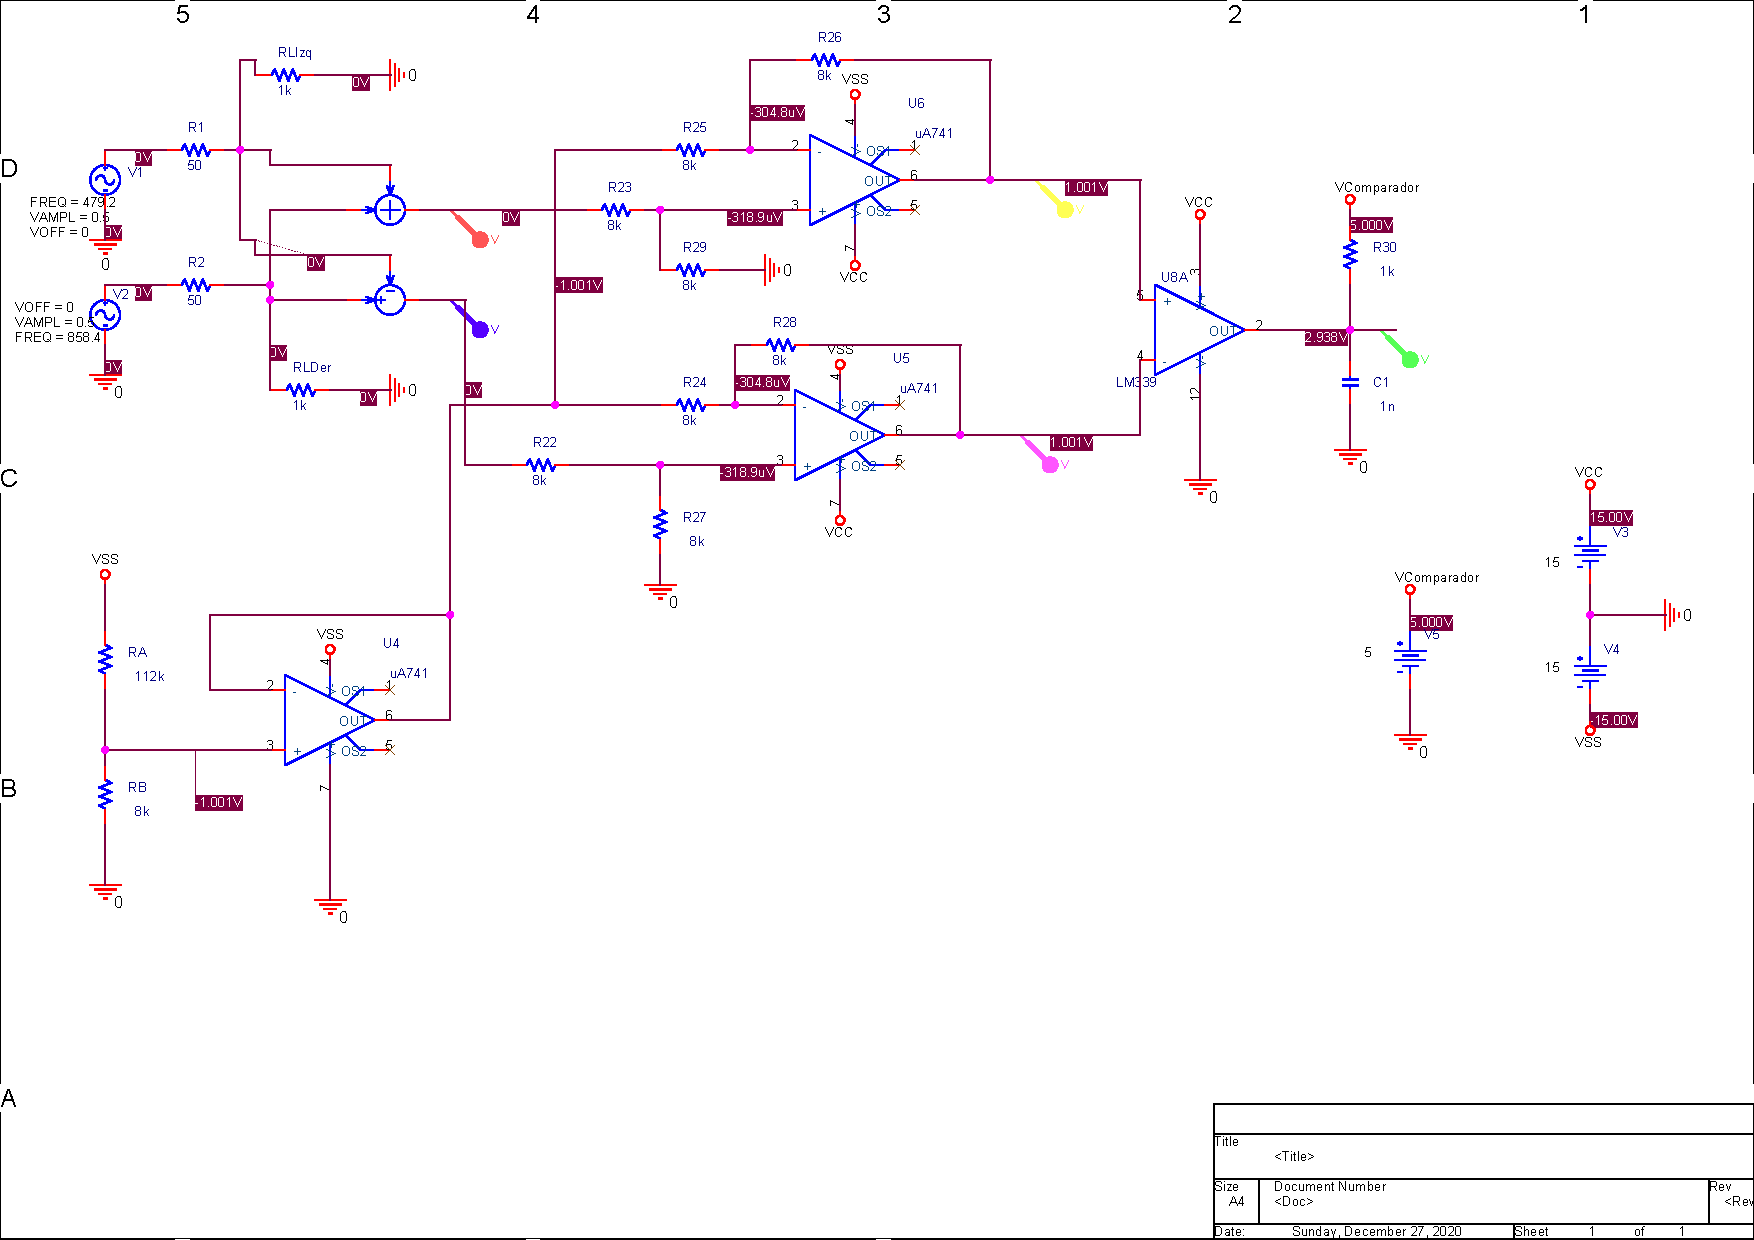
\includegraphics[scale=0.8,page=1,clip, trim=17cm 12cm 5.5cm 3cm]{images/problema_puntuable_6_sche.pdf}
    % izquierda,abajo,derecha,arriba
    \caption{Circuito comparador}
  \end{figure}

  Resuelto el tema del uso del A.O. comparador tenemos otro problema
  entre manos y es que el uso de una configuración no simétrica nos
  impide trabajar con todo el rango de valores que tienen nuestras
  señales ya que solo puede trabajar entre 0 y 5 voltios
  (señales TTL),   esto nos obliga añadir 3 amplificadores más y un divisor de tensión.
  
  Dos amplificadores los usaremos para sumar (si están en
  configuración diferncial restar) una componente de continua a la
  señal lo cual la desplaza positiva o negativamente según el signo de
  la entrada, en este caso vamos a introducir una señal con valor de
  $-1$ (por lo tanto usaremos uan configuración diferencial), esto nos permitirá trabajar en el rango de 0 a 5 sin
  problemas.

    \begin{figure}[H]
    \centering  
    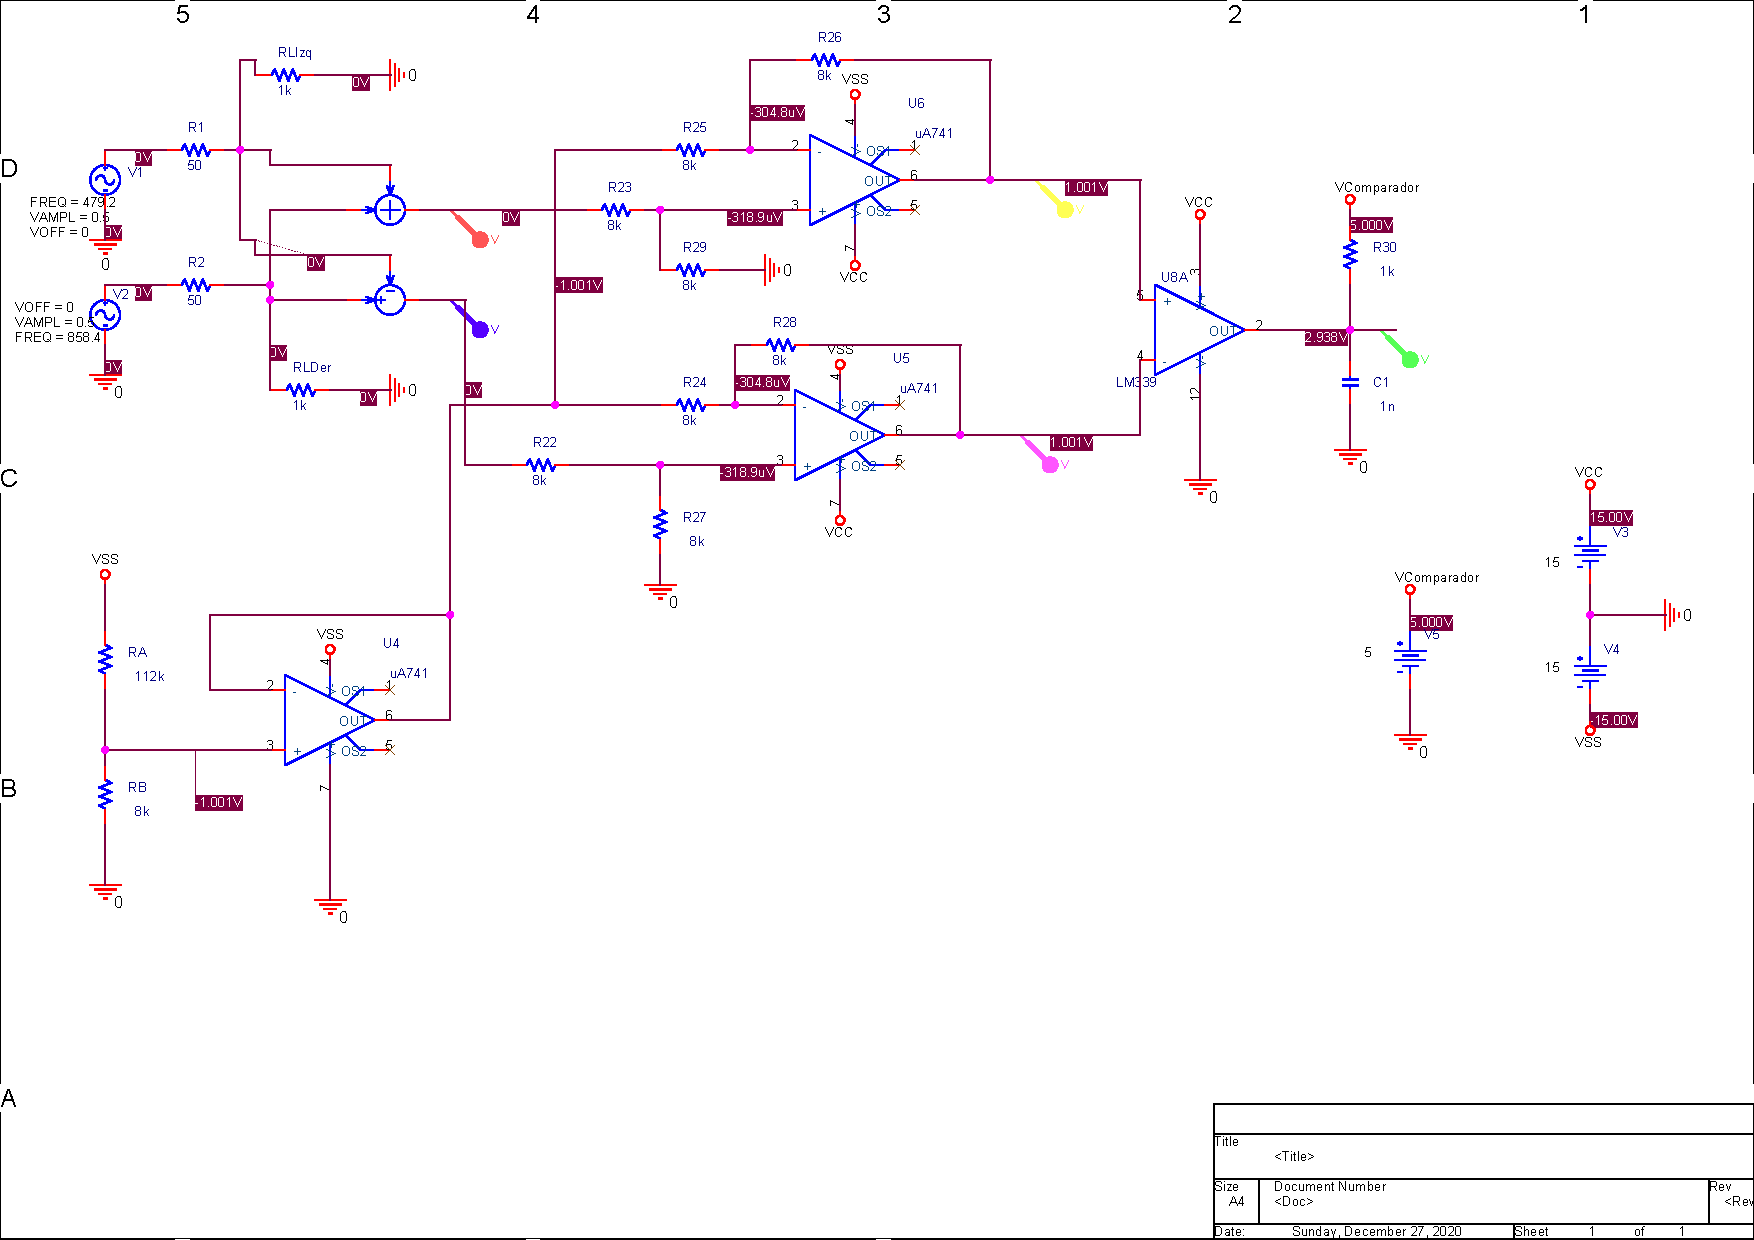
\includegraphics[scale=0.8,page=1,clip, trim=12cm 11.5cm 12cm 0.5cm]{images/problema_puntuable_6_sche.pdf}
    % izquierda,abajo,derecha,arriba
    \caption{Amplificadores en configuración diferencial}
  \end{figure}

  La suma de una componente de continua en nuestro circuito sin el uso
  de fuentes de tensión externas puede hacerse con la alimentación
  simétrica del circuito base, un divisor de tensión y un amplificador
  operacional, la alimentación simétrica nos proporciona un tensión de
  -15 voltios, esta se dividirá en dos resistencias una de $112k\Omega$
  y otra de $8k\Omega$ lo que nos da $-1 V$ de salida pero este juego
  de tensiones nos va a costar el uso de un amplificador más como
  buffer para adapatar las impedancias porque incluso cuando nuestros
  amplificadores suma tienen una impedancia muy alta la resistencia de
  $112k\Omega$ tiene un gran impacto.

  Divisor de tensión:
  \begin{equation}
    V_{out} = \dfrac{R_2}{R_1+R_2}\cdot V_{in}
  \end{equation}
    \begin{equation}
    1 = \dfrac{8k}{R_1+8k}\cdot 15
  \end{equation}
      \begin{equation}
        R_1 = 112k \Omega
    \end{equation}

      \begin{figure}[H]
    \centering  
    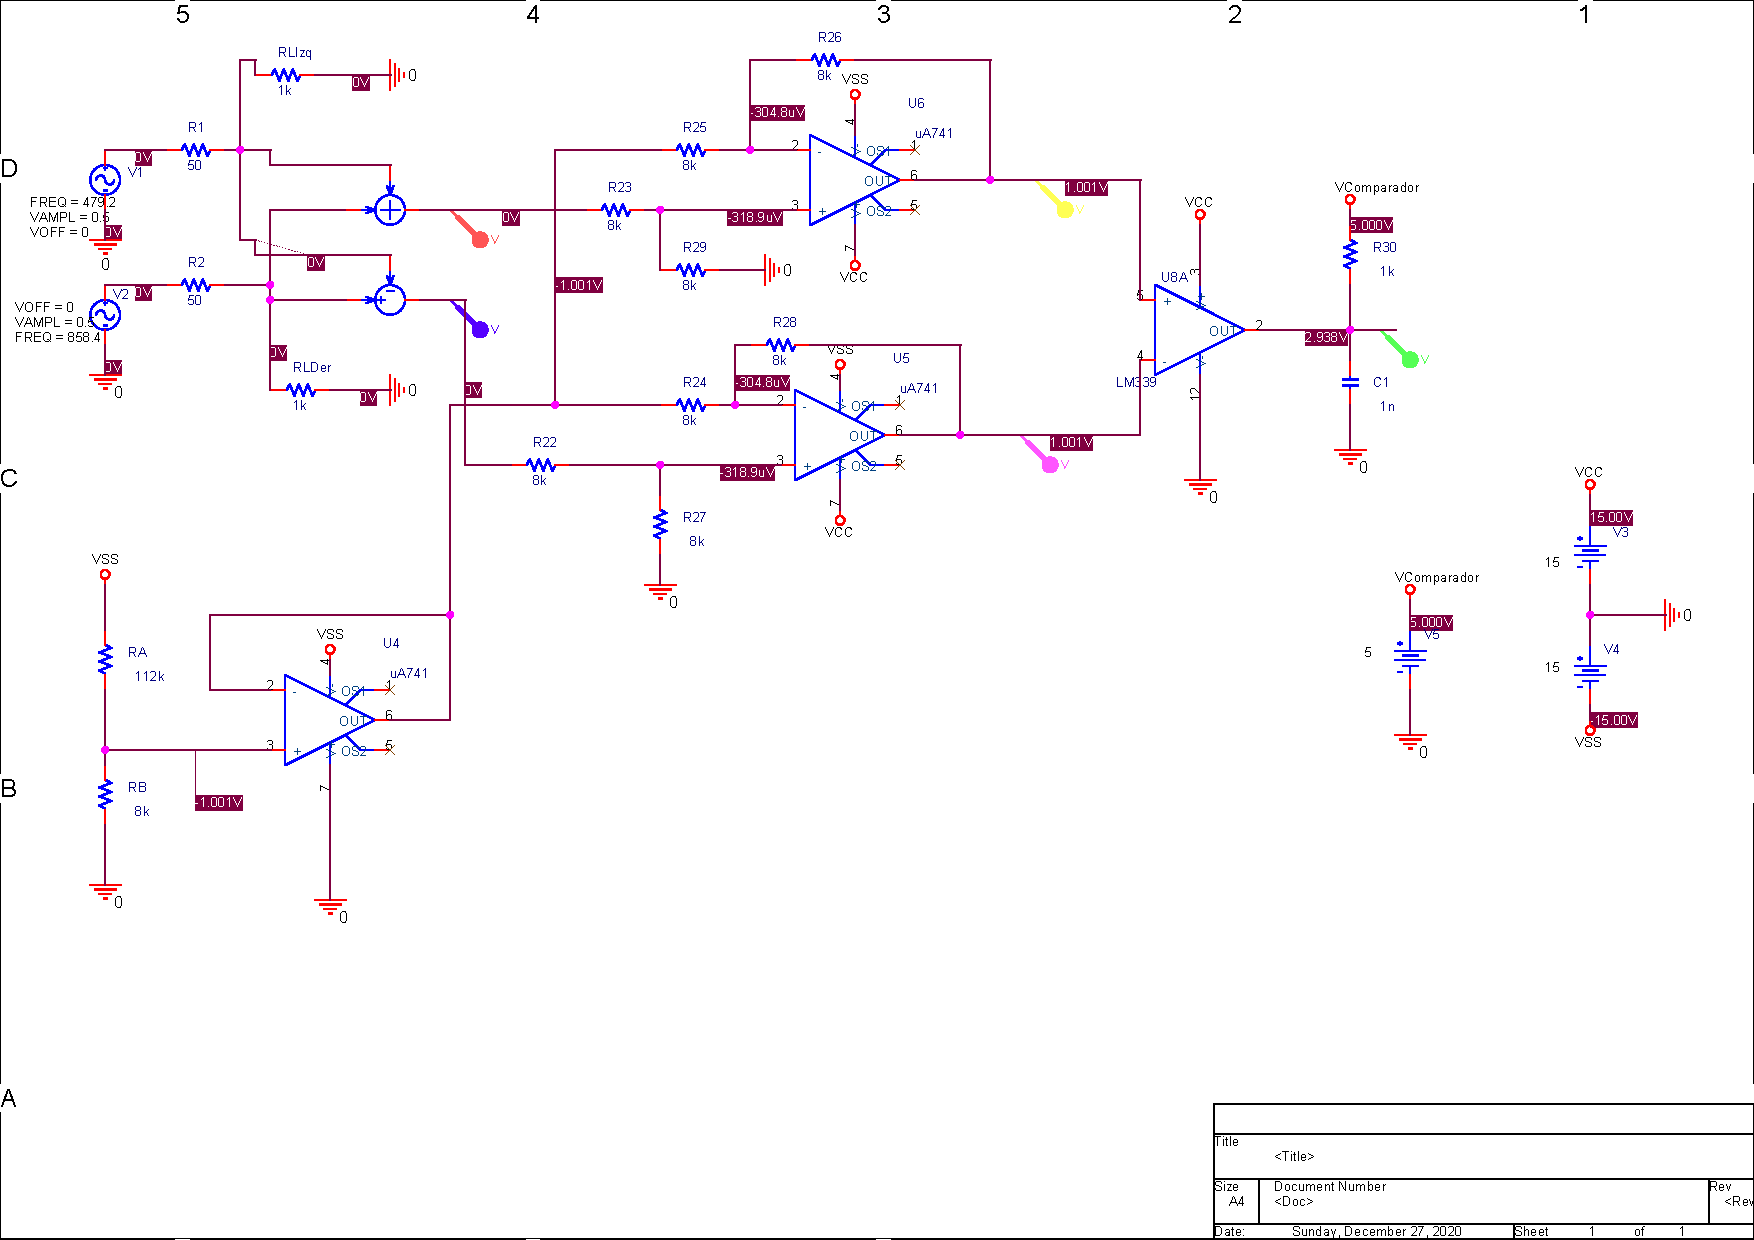
\includegraphics[scale=0.8,page=1,clip, trim=1cm 5cm 22cm 8cm]{images/problema_puntuable_6_sche.pdf}
    % izquierda,abajo,derecha,arriba
    \caption{Buffer}
  \end{figure}

    Como podemos observar con el divisor de tensión hemos conseguido
    casi un tensión de $-1V$.

      \begin{figure}[H]
    \centering  
    \includegraphics[scale=0.5,page=4]{images/problema_puntuable_6_gráficas.pdf}
    % izquierda,abajo,derecha,arriba
    \caption{Salida sin componente de continua}
  \end{figure}

      \begin{figure}[H]
    \centering  
    \includegraphics[scale=0.5,page=3]{images/problema_puntuable_6_gráficas.pdf}
    % izquierda,abajo,derecha,arriba
    \caption{Salida con componente de continua}
  \end{figure}
  
    Como resultado tenemos el siguiente circuito.

      \begin{figure}[H]
    \centering  
    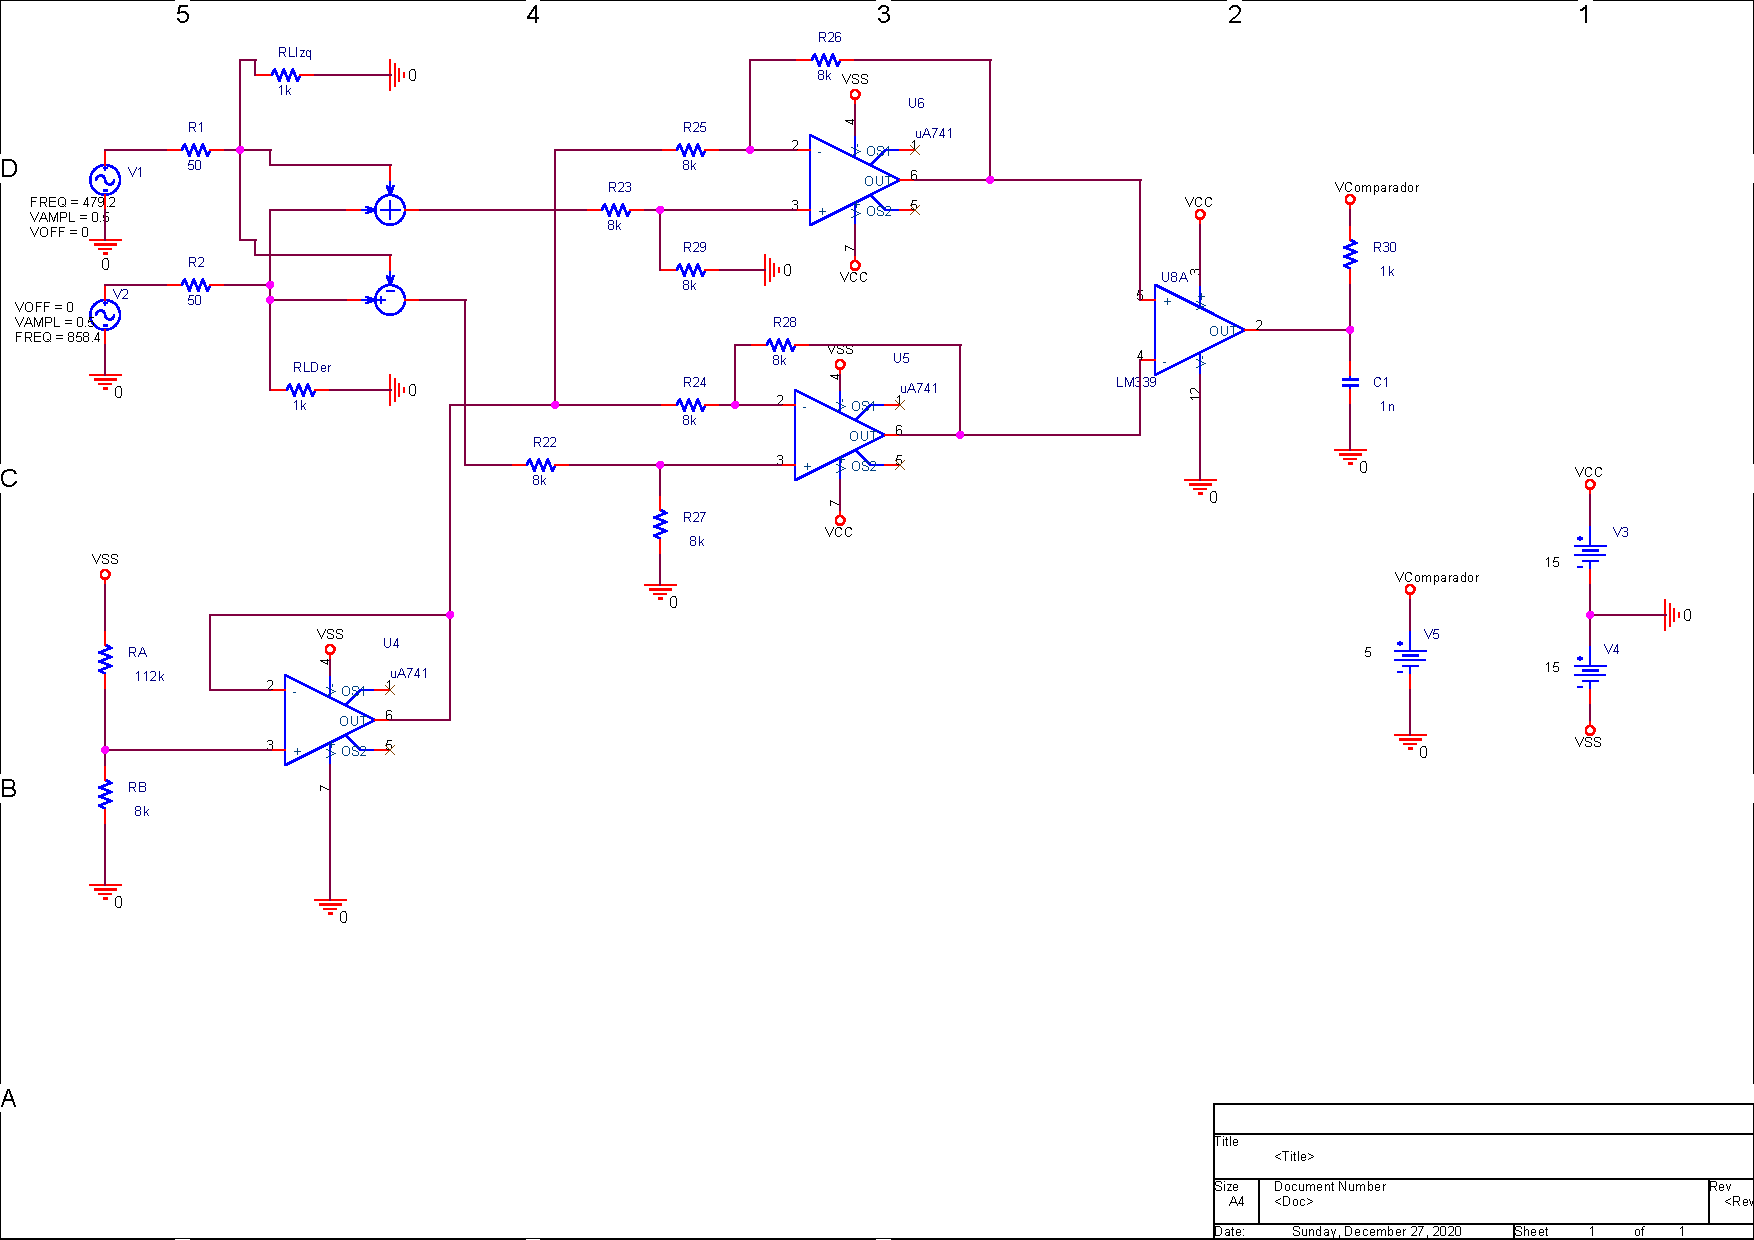
\includegraphics[scale=0.6,page=1,clip, trim=1cm 5cm 1cm 0.45cm]{images/problema_puntuable_6_schee.pdf}
    % izquierda,abajo,derecha,arriba
    \caption{Esquema del circuito completo}
  \end{figure}
  
    y su respectiva salida en el domino del tiempo.

       \begin{figure}[H]
    \centering  
    \includegraphics[scale=0.5,page=5]{images/problema_puntuable_6_gráficas.pdf}
    % izquierda,abajo,derecha,arriba
    \caption{Salida del comparador}
  \end{figure}
  
    
    Cuando la señal suma (rojo) es mayor que la señal resta (verde)
    tenemos una tensión de 5 voltios o lo que es lo mismo un 1 lógico,
    un verdadero, cuando la señal es menor casi cero voltios lo que se
    traduce en un cero lógico. Es importante destacar que la
    frecuencia de la salida es igual a la frecuencia de la menor de
    las señales.

    En la siguiente gráfica se puede ver la componente de continua y
    la salida.

          \begin{figure}[H]
    \centering  
    \includegraphics[scale=0.5,page=1]{images/problema_puntuable_6_gráficas.pdf}
    % izquierda,abajo,derecha,arriba
    \caption{Señales sin componente de continua, con componente de
      continua y salida del comparador}
  \end{figure}
  
}